
\documentclass{beamer}

\usetheme{focus} % see https://github.com/elauksap/focus-beamertheme
% Add option [numbering=none] to disable the footer progress bar
% Add option [numbering=fullbar] to show the footer progress bar as always full with a slide count

\usepackage{booktabs} % Required for better table rules
\usepackage{bm,times}

\usepackage{tikz}
\usetikzlibrary{decorations.pathreplacing,calc}

\newcommand{\tikzmark}[1]{\tikz[overlay,remember picture] \node (#1) {};}

\newcommand{\eps}{\epsilon}
\newcommand{\RR}{\mathbb{R}}

\newcommand{\grad}{\nabla}
\newcommand{\Div}{\nabla\cdot}
\newcommand{\trace}{\operatorname{tr}}

\newcommand{\hbn}{\hat{\mathbf{n}}}

\newcommand{\bb}{\mathbf{b}}
\newcommand{\be}{\mathbf{e}}
\newcommand{\bbf}{\mathbf{f}}
\newcommand{\bg}{\mathbf{g}}
\newcommand{\bn}{\mathbf{n}}
\newcommand{\br}{\mathbf{r}}
\newcommand{\bu}{\mathbf{u}}
\newcommand{\bv}{\mathbf{v}}
\newcommand{\bw}{\mathbf{w}}
\newcommand{\bx}{\mathbf{x}}

\newcommand{\bF}{\mathbf{F}}
\newcommand{\bV}{\mathbf{V}}
\newcommand{\bX}{\mathbf{X}}

\newcommand{\bxi}{\bm{\xi}}

\newcommand{\bzero}{\bm{0}}

\newcommand{\rhoi}{\rho_{\text{i}}}

\newcommand{\ip}[2]{\left(#1,#2\right)}

\newcommand{\mR}{R^{\bm{\oplus}}}
\newcommand{\iR}{R^{\bullet}}

\newcommand{\pp}{{\text{p}}}
\newcommand{\qq}{{\text{q}}}
\newcommand{\rr}{{\text{r}}}

\newcommand{\bus}{\bu|_s}


\title{Evolution of \\ ice sheet geometry \\ using Stokes dynamics}

%\subtitle{Subtitle}

\author{Ed Bueler}

\titlegraphic{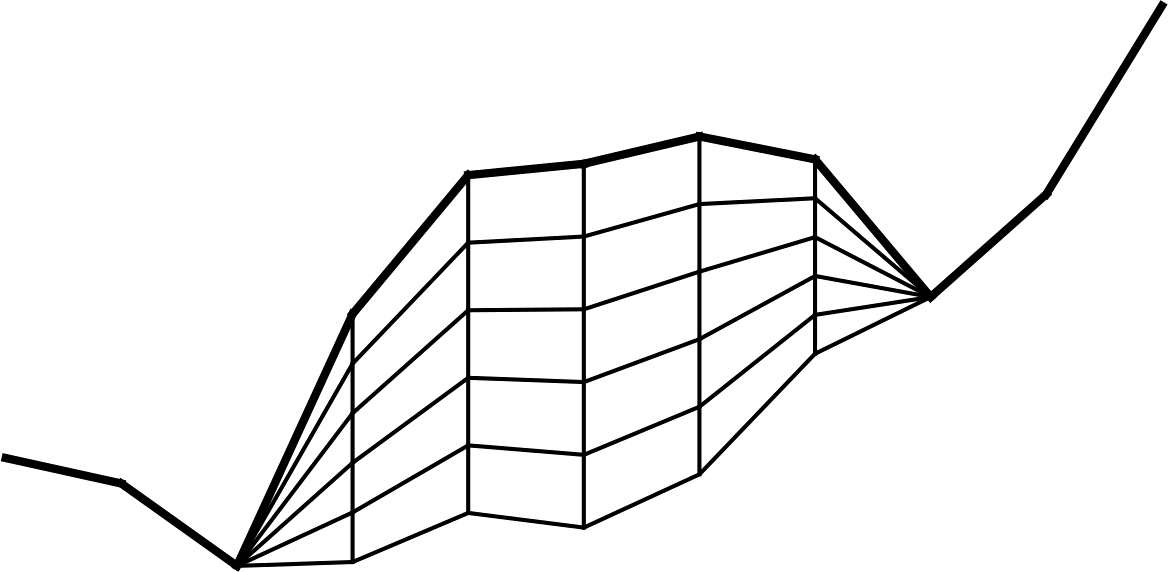
\includegraphics[width=0.7\textwidth]{figs/titleextruded.png} \\ \vspace{-3mm} 
\includegraphics[width=0.15\textwidth]{figs/uafbw.png}}

%\institute{University of Alaska Fairbanks}

\date{\phantom{foo} \bigskip \bigskip \bigskip \\ SIAM GS21 \\ with assistance from Lawrence Mitchell}


\begin{document}

\begin{frame}
	\maketitle
\end{frame}


\begin{frame}{the steady ice geometry problem (SIGP)}

\vspace{-2mm}
\begin{center}
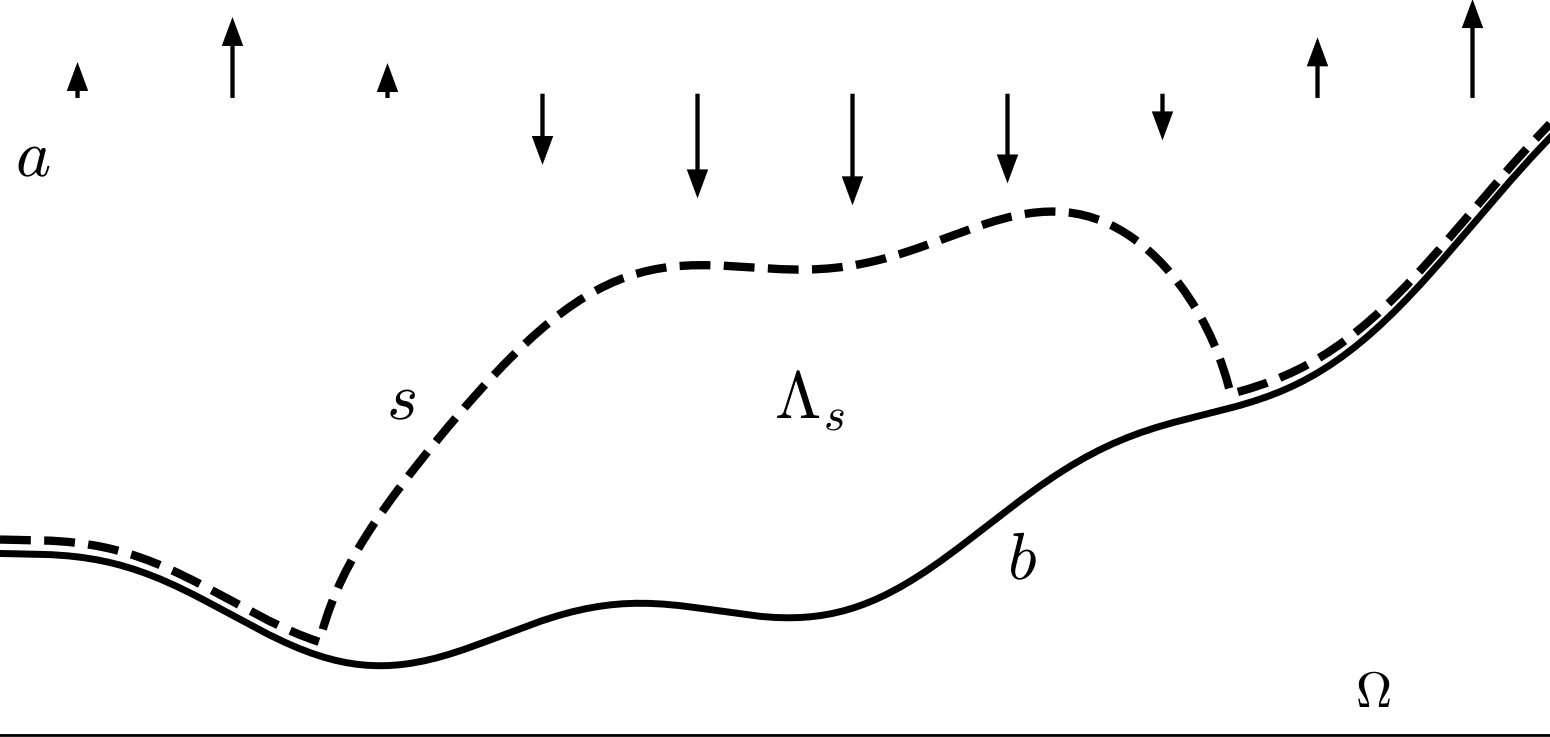
\includegraphics[width=0.7\textwidth]{figs/stokesdomain.png}
\end{center}

\vspace{-1mm}
\begin{itemize}
\item a non-shallow glacier interacting with the climate
    \begin{itemize}
    \item only the simplest such problem (nonsliding, isothermal)
    \item re~\emph{steady}: solve this and you can handle implicit steps too
    \end{itemize}
\item data given on fixed $\Omega \subset \RR^2$:
    \begin{itemize}
    \item climatic mass balance $a(x,y)$ \hfill $\gets$ \emph{steady climate}
    \item bed elevation $b(x,y)$
    \end{itemize}
\item determine: surface elevation $s(x,y)$ on $\Omega$ and domain $\Lambda_s \subset \RR^3$
\end{itemize}
\end{frame}


\begin{frame}{surface kinematical equation}

\begin{block}{steady surface kinematical equation (SKE)}
$$\bu|_s \cdot \bn_s + a=0$$
\end{block}

\begin{itemize}
\item $\bn_s = \left<-s_x,-s_y,1\right>$  \quad (normal to ice surface; upward)
\item \emph{on} the ice surface, in steady-state there is balance (SKE) between motion and climatic mass balance
\item \emph{off} the ice we know $a\le 0$ in steady state
\item for all of this talk: $s=b$ where ice is not present
\end{itemize}
\end{frame}


\begin{frame}{SIGP strong form}

\begin{itemize}
\item \alert{a nonlinear complementarity problem (NCP) for $s$ coupled to Stokes problem for $\bu,p$:}

\vspace{-5mm}

\begin{align*}
s - b &\ge 0 && \text{on $\Omega$} & \tikzmark{ncptop} \\
- \bu|_s \cdot \bn_s - a &\ge 0 && \text{''} \\
(s - b) (- \bu|_s \cdot \bn_s - a) &= 0 && \text{''} & \tikzmark{ncpbot} \\
- \nabla \cdot \left(2 \nu_\eps\, D\bu\right) + \nabla p - \rhoi \mathbf{g} &= \bzero && \text{on $\Lambda_s$} & \tikzmark{gstop} \\
\nabla \cdot \bu &= 0 && \text{''} \\
\bu &= \bzero && \text{on $\Gamma_0$ \quad (ice base)} \\
\left(2 \nu_\eps D\bu - pI\right) \bn &= \bzero && \text{on $\partial \Lambda_s \setminus \Gamma_0$} & \tikzmark{gsbot}
\end{align*}

\begin{tikzpicture}[overlay, remember picture]
\draw[decoration={brace,amplitude=0.4em},decorate,ultra thick] ([xshift=-7mm]ncptop.north east) node[right=8mm,below=3mm] {NCP} -- ([xshift=-7mm]ncpbot.east);
\end{tikzpicture}

\begin{tikzpicture}[overlay, remember picture]
\draw[decoration={brace,amplitude=0.4em},decorate,ultra thick] ([xshift=-7mm]gstop.north east) node[right=10mm,below=6mm] {Stokes} -- ([xshift=-7mm]gsbot.east);
\end{tikzpicture}

\vspace{-8mm}

    \begin{itemize}
    \item plus Glen-law effective viscosity with $\text{p}=(1/\text{n})+1(=4/3)$:
      $$\nu_\eps = \frac{1}{2} B_n \left(|D\bu|^2 + \eps\, D_0^2\right)^{(\pp-2)/2}$$
    \end{itemize}
\item SIGP is a free-boundary problem for $s$ defined on $\Omega$
\end{itemize}
\end{frame}


\begin{frame}{existing ice sheet models}

\begin{itemize}
\item almost no one is solving the SIGP directly, or doing implicit time-stepping
    \begin{itemize}
    \item except Wirbel \& Jarosch \cite{WirbelJarosch2020} \dots nonscalable, w.~``fake ice''
    \end{itemize}
\item what are people doing instead?
    \begin{itemize}
    \item \alert{explicit time-stepping with $s \ge b$ enforced by truncation} (below)
    \end{itemize}
\end{itemize}

\medskip
\begin{columns}
    \column{0.8\textwidth}
        \hfill 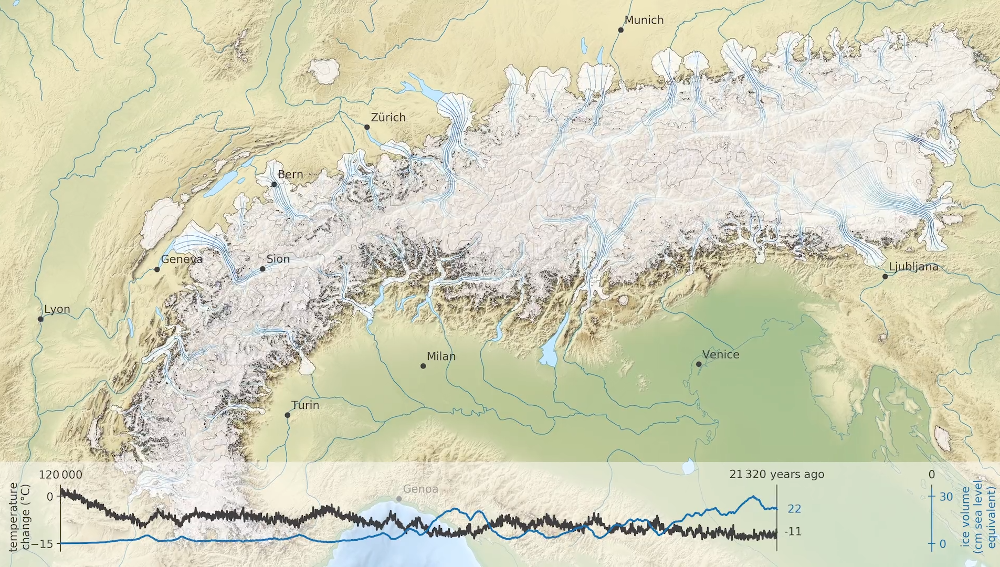
\includegraphics[width=0.8\textwidth]{figs/seguinot.png}
    \column{0.2\textwidth}
        \scriptsize \emph{show clip of PISM run by Julien Seguinot}
\end{columns}
\end{frame}


\begin{frame}{coupling via operator}

\begin{block}{ice dynamics operator}
$\Phi : s \mapsto \bus \cdot \bn_s$

\vspace{-3mm}

\hfill 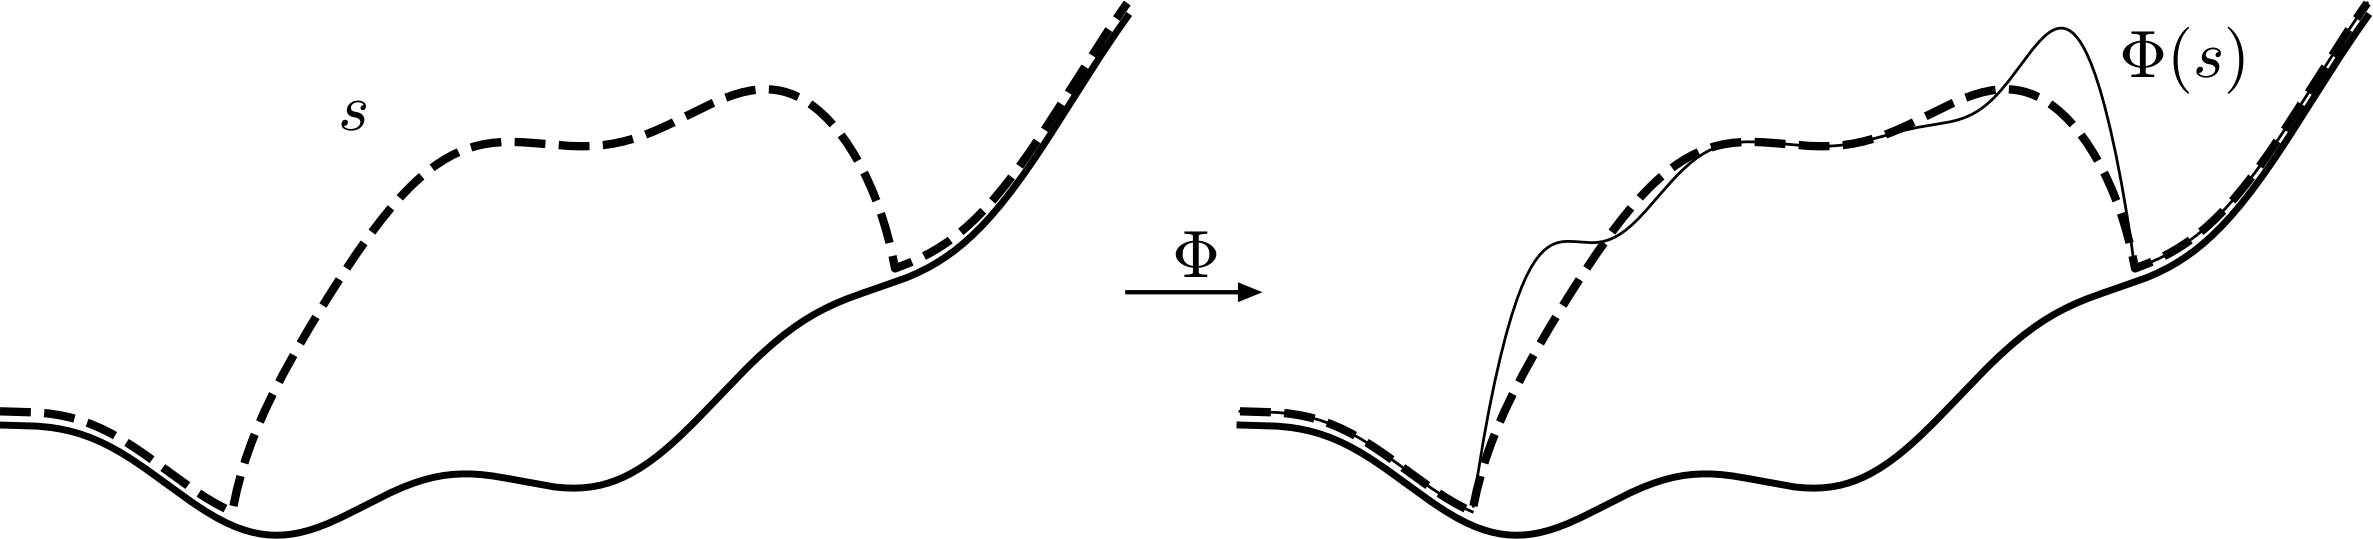
\includegraphics[width=0.75\textwidth]{figs/idoaction.png}
\end{block}

\begin{itemize}
\item to compute $\Phi(s)$, solve Stokes (weak form) problem
    $$F_{\Lambda_s}(\bu,p)[\bv,q] = \int_{\Lambda_s} 2 \nu_\eps D\bu : D\bv - p \Div\bv - (\Div\bu) q - \rhoi \bg \cdot \bv\,d\bx = 0$$
over $W_0^{1,\pp}(\Lambda_s)^3 \times L^\qq(\Lambda_s)$ and extract trace $\bus$

\medskip
    \begin{itemize}
    \item optimal solver already exists for this problem (Isaac et al \cite{IsaacStadlerGhattas2015})
    \end{itemize}
\item extend by zero so $\Phi(s)$ is defined on all of $\Omega$
\end{itemize}

\end{frame}


\begin{frame}{SIGP weak form is a variational inequality}

\begin{itemize}
\item using $\Phi$ gives clean NCP over $\Omega$:
\begin{align*}
s - b &\ge 0 \\
- \Phi(s) - a &\ge 0 \\
(s - b) (- \Phi(s) - a) &= 0
\end{align*}

\item well-known fact: \quad  NCP (strong form) $\leftrightarrow$ VI (weak form)
\item find $s \in \mathcal{K} = \{r \ge b\}$ so that
    $$\hspace{10mm} F(s)[r - s] \ge \ip{a}{r-s} \hspace{10mm} (\ast)$$
for all $r \in \mathcal{K}$, where
    $$F(s)[w] = - \int_\Omega \Phi(s)\, w \,dx dy$$
    \begin{itemize}
    \item whether VI problem $(\ast)$ is well-posed is open, but the SIA version has an existence proof (Jouvet \& Bueler \cite{JouvetBueler2012})
    \end{itemize}
\end{itemize}

\end{frame}


\begin{frame}{goal: robust and optimal SIGP solver}

\begin{block}{goal}
given triangulation $\mathcal{T}$ of $\Omega$, and $P_1$ FE space $\mathcal{V}^h \subset W^{1,\qq}(\Omega)$, solve SIGP VI

$$F(s^h)[r^h - s^h] \ge \ip{a}{r^h-s^h}$$

for admissible $s^h$ using solutions of Glen-Stokes problem $F_{\Lambda_{s^h}}(\bu^h,p^h)=0$ to evaluate $\Phi(s)=\bu|_s\cdot\bn_s$ and $F(s)[w] =- \int_\Omega \Phi(s)\, w $
\end{block}

\begin{itemize}
\item seeking a solver which is:
    \begin{itemize}
    \item \alert{robust}
    \item \alert{optimal} over $m$ degrees of freedom in $\mathcal{V}^h$: work is $O(m)$
    \end{itemize}
\item optimal requires multigrid
\end{itemize}
\end{frame}


\begin{frame}{new method}

\begin{itemize}
\item FIXME \cite{BuelerMitchell2022}
\end{itemize}

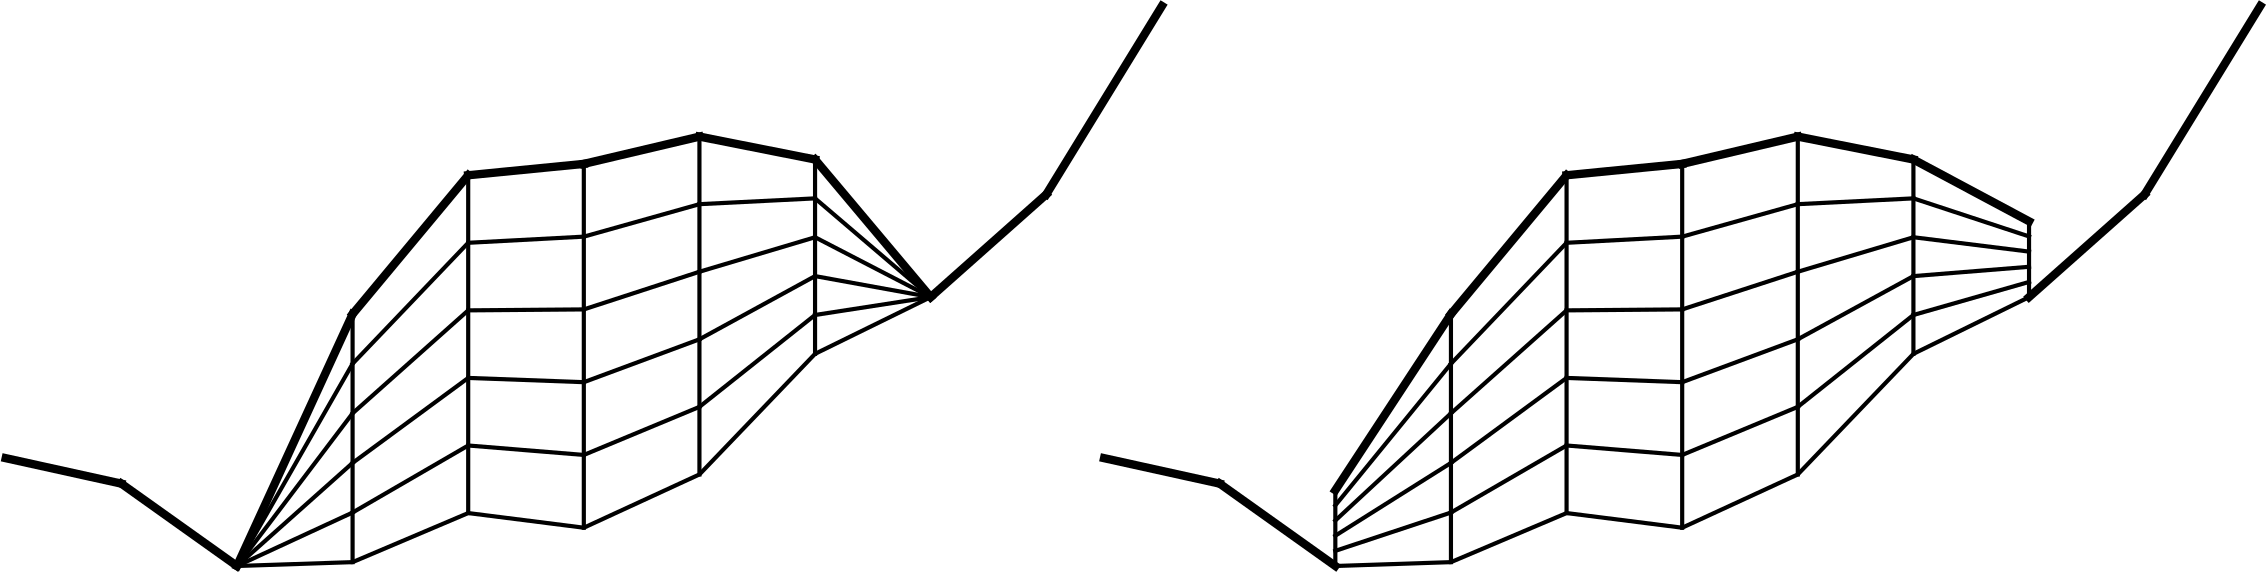
\includegraphics[width=0.8\textwidth]{figs/extruded.png}
\end{frame}


\begin{frame}{extra}
 NCP is a barrier to exact numerical mass conservation \cite{Bueler2021conservation}
\end{frame}

%\begin{block}{Block}
%\begin{alertblock}{Alert block}
%	\pause % Automatically creates a new "page" split between the above and above + below
%	\begin{exampleblock}{Example block}


%\begin{frame}{Columns}
%	\begin{columns}
%		\column{0.5\textwidth}
%			This text
%		\column{0.5\textwidth}
%			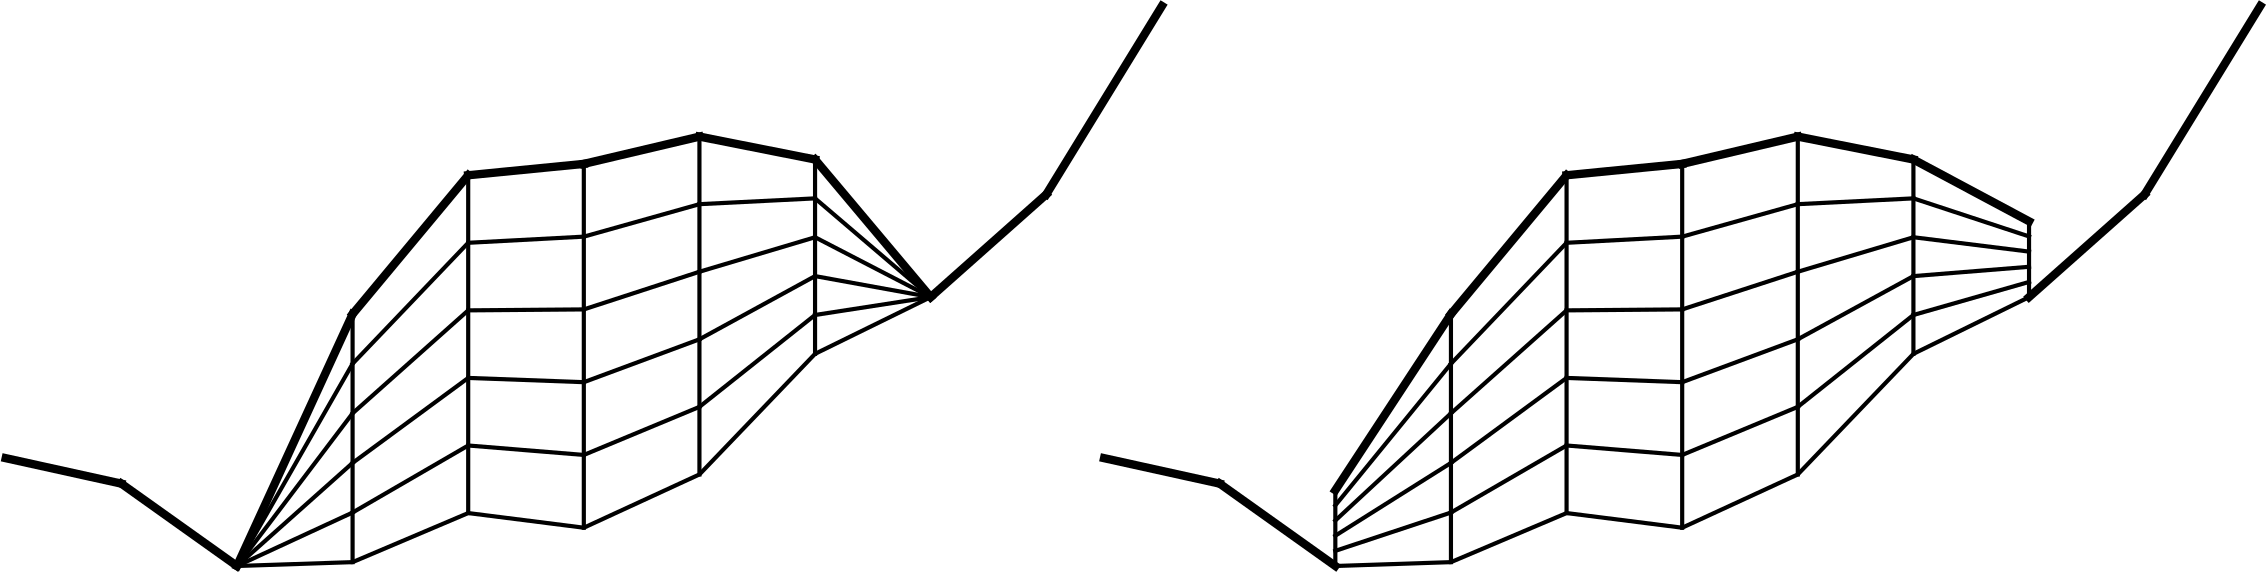
\includegraphics[width=\linewidth]{figs/extruded.png}
%	\end{columns}
%\end{frame}


\appendix

\begin{frame}{References}

%\bibliography{../paper/msg.bib}
%\bibliographystyle{plain}

\begin{thebibliography}{1}
\bibitem{Bueler2021conservation}
E.~Bueler. \textbf{Conservation laws for free-boundary fluid layers.} {\em SIAM J. Appl. Math.}, to appear.

\bibitem{BuelerMitchell2022}
E.~Bueler and L.~Mitchell. \textbf{Multilevel computation of glacier geometry from Stokes dynamics.} in preparation

\bibitem{IsaacStadlerGhattas2015}
T.~Isaac, G.~Stadler, and O.~Ghattas.  \textbf{Solution of nonlinear Stokes equations discretized by high-order finite elements on nonconforming and anisotropic meshes, with application to ice sheet dynamics.} {\em SIAM J. Sci. Comput.}, 37(6):B804--B833, 2015.

\bibitem{JouvetBueler2012}
G.~Jouvet and E.~Bueler. \textbf{Steady, shallow ice sheets as obstacle problems: well-posedness and finite element approximation.} {\em SIAM J. Appl. Math.}, 72(4):1292--1314, 2012.

\bibitem{WirbelJarosch2020}
A.~Wirbel and A.~H. Jarosch. \textbf{Inequality-constrained free-surface evolution in a full {S}tokes ice flow model (\textit{evolve\_glacier v1.1}).} {\em Geoscientific Model Development}, 13(12):6425--6445, 2020.
\end{thebibliography}

\end{frame}


\end{document}
